\chapter{元编程}
\label{cp:meta}

\section{构建系统}

\textbf{构建系统是开发流程的基础}。其作用是\textbf{通过一系列规则和指令自动化地将源代码编译为可执行文件、库文件或者其他输出目标}。\textit{在小型项目中,手动编译和链接源文件可能已经足够,但是随着项目规模的增长,源文件之间的依赖关系变得错综复杂,手工编译不仅耗时耗力,还容易出错。}这时,构建工具便显得尤为重要。构建工具如\texttt{Makefile}和\texttt{CMake}可以自动处理文件依赖,编译、链接源文件,并支持跨平台的构建需求,使项目的开发流程更加高效和可靠。

\subsection{Makefile}

\textbf{Makefile是Linux系统中最早期且广泛使用的构建工具之一}。它依赖于\textit{GNU Make}工具,通过\textit{定义一组目标(target)、依赖关系(dependencies)和规则(rules),自动化地完成编译过程}。典型的\texttt{Makefile}文件通常由多个部分组成,描述了从源文件生成目标文件的过程。\\

我们只能给出一个简单的\texttt{Makefile}示例,如代码\ref{listing:makefile}所示。

\begin{longlisting}
    \begin{minted}{make}
CC = gcc
CFLAGS = -Wall -g

SRCS = main.c utils.c
OBJS = $(SRCS:.c=.o)
TARGET = program

$(TARGET): $(OBJS)
    $(CC) $(CFLAGS) -o $(TARGET) $(OBJS)

%.o: %.c
    $(CC) $(CFLAGS) -c $< -o $@

clean:
    rm -f $(OBJS) $(TARGET)
    \end{minted}
    \caption{Makefile编译C项目的示例}
    \label{listing:makefile}
\end{longlisting}

在这个Makefile中,\texttt{CC}表示\textit{编译器(此处为gcc)},\texttt{CFLAGS}定义了\textit{编译器的选项},包括显示所有警告(\texttt{-Wall})和生成调试信息(\texttt{-g})。\texttt{SRCS}列出了\textit{所有源文件},而\texttt{OBJS}则是由源文件生成的目标文件。\texttt{\$(TARGET)}是最终的可执行文件。\\

执行\texttt{make}命令,\texttt{Make}就会\textit{自动计算每个目标文件的依赖,并根据规则编译源代码}。clean命令用于清理生成的目标文件和可执行文件。\\

下面我们给出一个使用\texttt{Makefile}编译一个Hello World C程序的示例,如代码\ref{listing:makefile-example}所示。

\begin{longlisting}
    \begin{minted}{bash}
# 安装 make 工具
sudo apt install build-essential -y

# 假设目录中已有了 helloworld.c 文件
# 创建 Makefile 文件
echo 'CC=gcc
CFLAGS=-Wall -Wextra -std=c99

all: helloworld

helloworld: helloworld.c
	$(CC) $(CFLAGS) -o helloworld helloworld.c

clean:
	rm -f helloworld' >> Makefile

# 执行 make 命令
make
## 看到 gcc -Wall -Wextra -std=c99 -o helloworld helloworld.c 说明编译成功
chmod +x helloworld
./helloworld
## Hello, World!

# 清理编译文件
make clean
## rm -f helloworld 此时 helloworld 文件已被删除
    \end{minted}
    \caption{使用Makefile编译Hello World C程序}
    \label{listing:makefile-example}
\end{longlisting}

具体运行效果见图\ref{fig:makefile-example}。

\begin{figure}[!htbp]
    \centering
    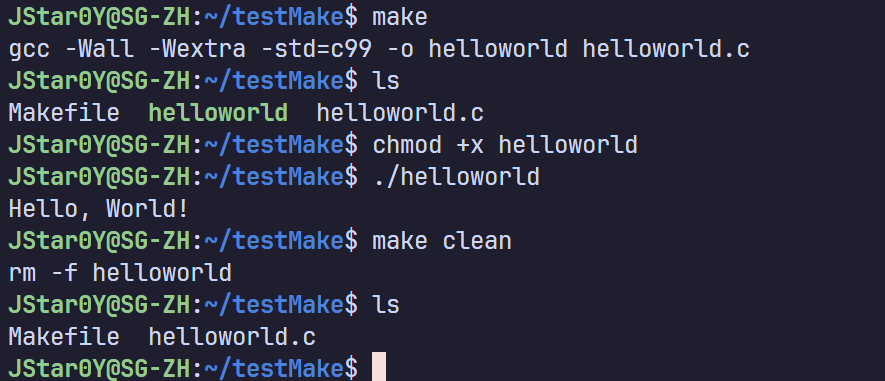
\includegraphics[width=0.8\textwidth]{Figures/make.png}
    \caption{使用Makefile编译Hello World C程序的运行效果}
    \label{fig:makefile-example}
\end{figure}

\textbf{Make的缺点显而易见。}虽然Makefile的简单、灵活和易于扩展使其在许多项目中被广泛使用。然而,\textbf{当项目变得更加复杂且跨平台需求增多时,Makefile的局限性开始显现。}特别是,当项目需要在不同的操作系统或编译器之间切换时,手动管理Makefile的复杂性变得不可控。

\subsection{CMake}

\textbf{CMake是一款开源的跨平台构建工具},它的设计初衷是为了解决Makefile的跨平台问题。在Linux系统中,\textbf{CMake生成Makefile},而\textbf{在Windows上,它可以生成Visual Studio的解决方案文件,或者也生成Makefile}。CMake的核心思想是将\textit{构建过程抽象化,通过CMake脚本定义项目的构建逻辑,使得同一套脚本可以在不同平台上复用。}也就是说,\textbf{CMake是一个构建系统生成器},它可以根据用户提供的配置信息生成适用于不同平台的构建系统。而\textit{CMake本身的配置是更为简单和方便的}(至少个人感觉)。\\

\textit{CMakeLists.txt}文件是CMake的核心配置文件,用于定义项目的构建步骤。我们在夏季小学期的实验中,就用了CMake来构建我们的项目。其\texttt{CMakeList.txt}的配置如代码\ref{listing:cmake}所示。

\begin{longlisting}
    \begin{minted}{cmake}
cmake_minimum_required(VERSION 3.12)
project(Game)

set(CMAKE_CXX_STANDARD 17)
set(CMAKE_CXX_FLAGS "${CMAKE_CXX_FLAGS} -fexec-charset=GBK -static-libstdc++ -static-libgcc -g")

file(GLOB SOURCES "src/*.cpp")

include_directories(${PROJECT_SOURCE_DIR}/include)

add_executable(Game ${SOURCES})
    \end{minted}
    \caption{CMake配置文件示例}
    \label{listing:cmake}
\end{longlisting}

在这个CMake配置文件中,\texttt{cmake\_minimum\_required}指定了CMake的最低版本要求,\texttt{project}定义了项目的名称。接着,\texttt{set}命令定义了\textit{编译器标准和编译选项},\texttt{file}命令用于\textit{查找源文件},\texttt{include\_directories}命令用于\textit{指定头文件目录},\texttt{add\_executable}命令用于\textit{定义可执行文件}。\\

请看\texttt{CMake}在我们具体的项目中的使用,如图\ref{fig:cmake}所示。

\begin{figure}[!htbp]
    \centering
    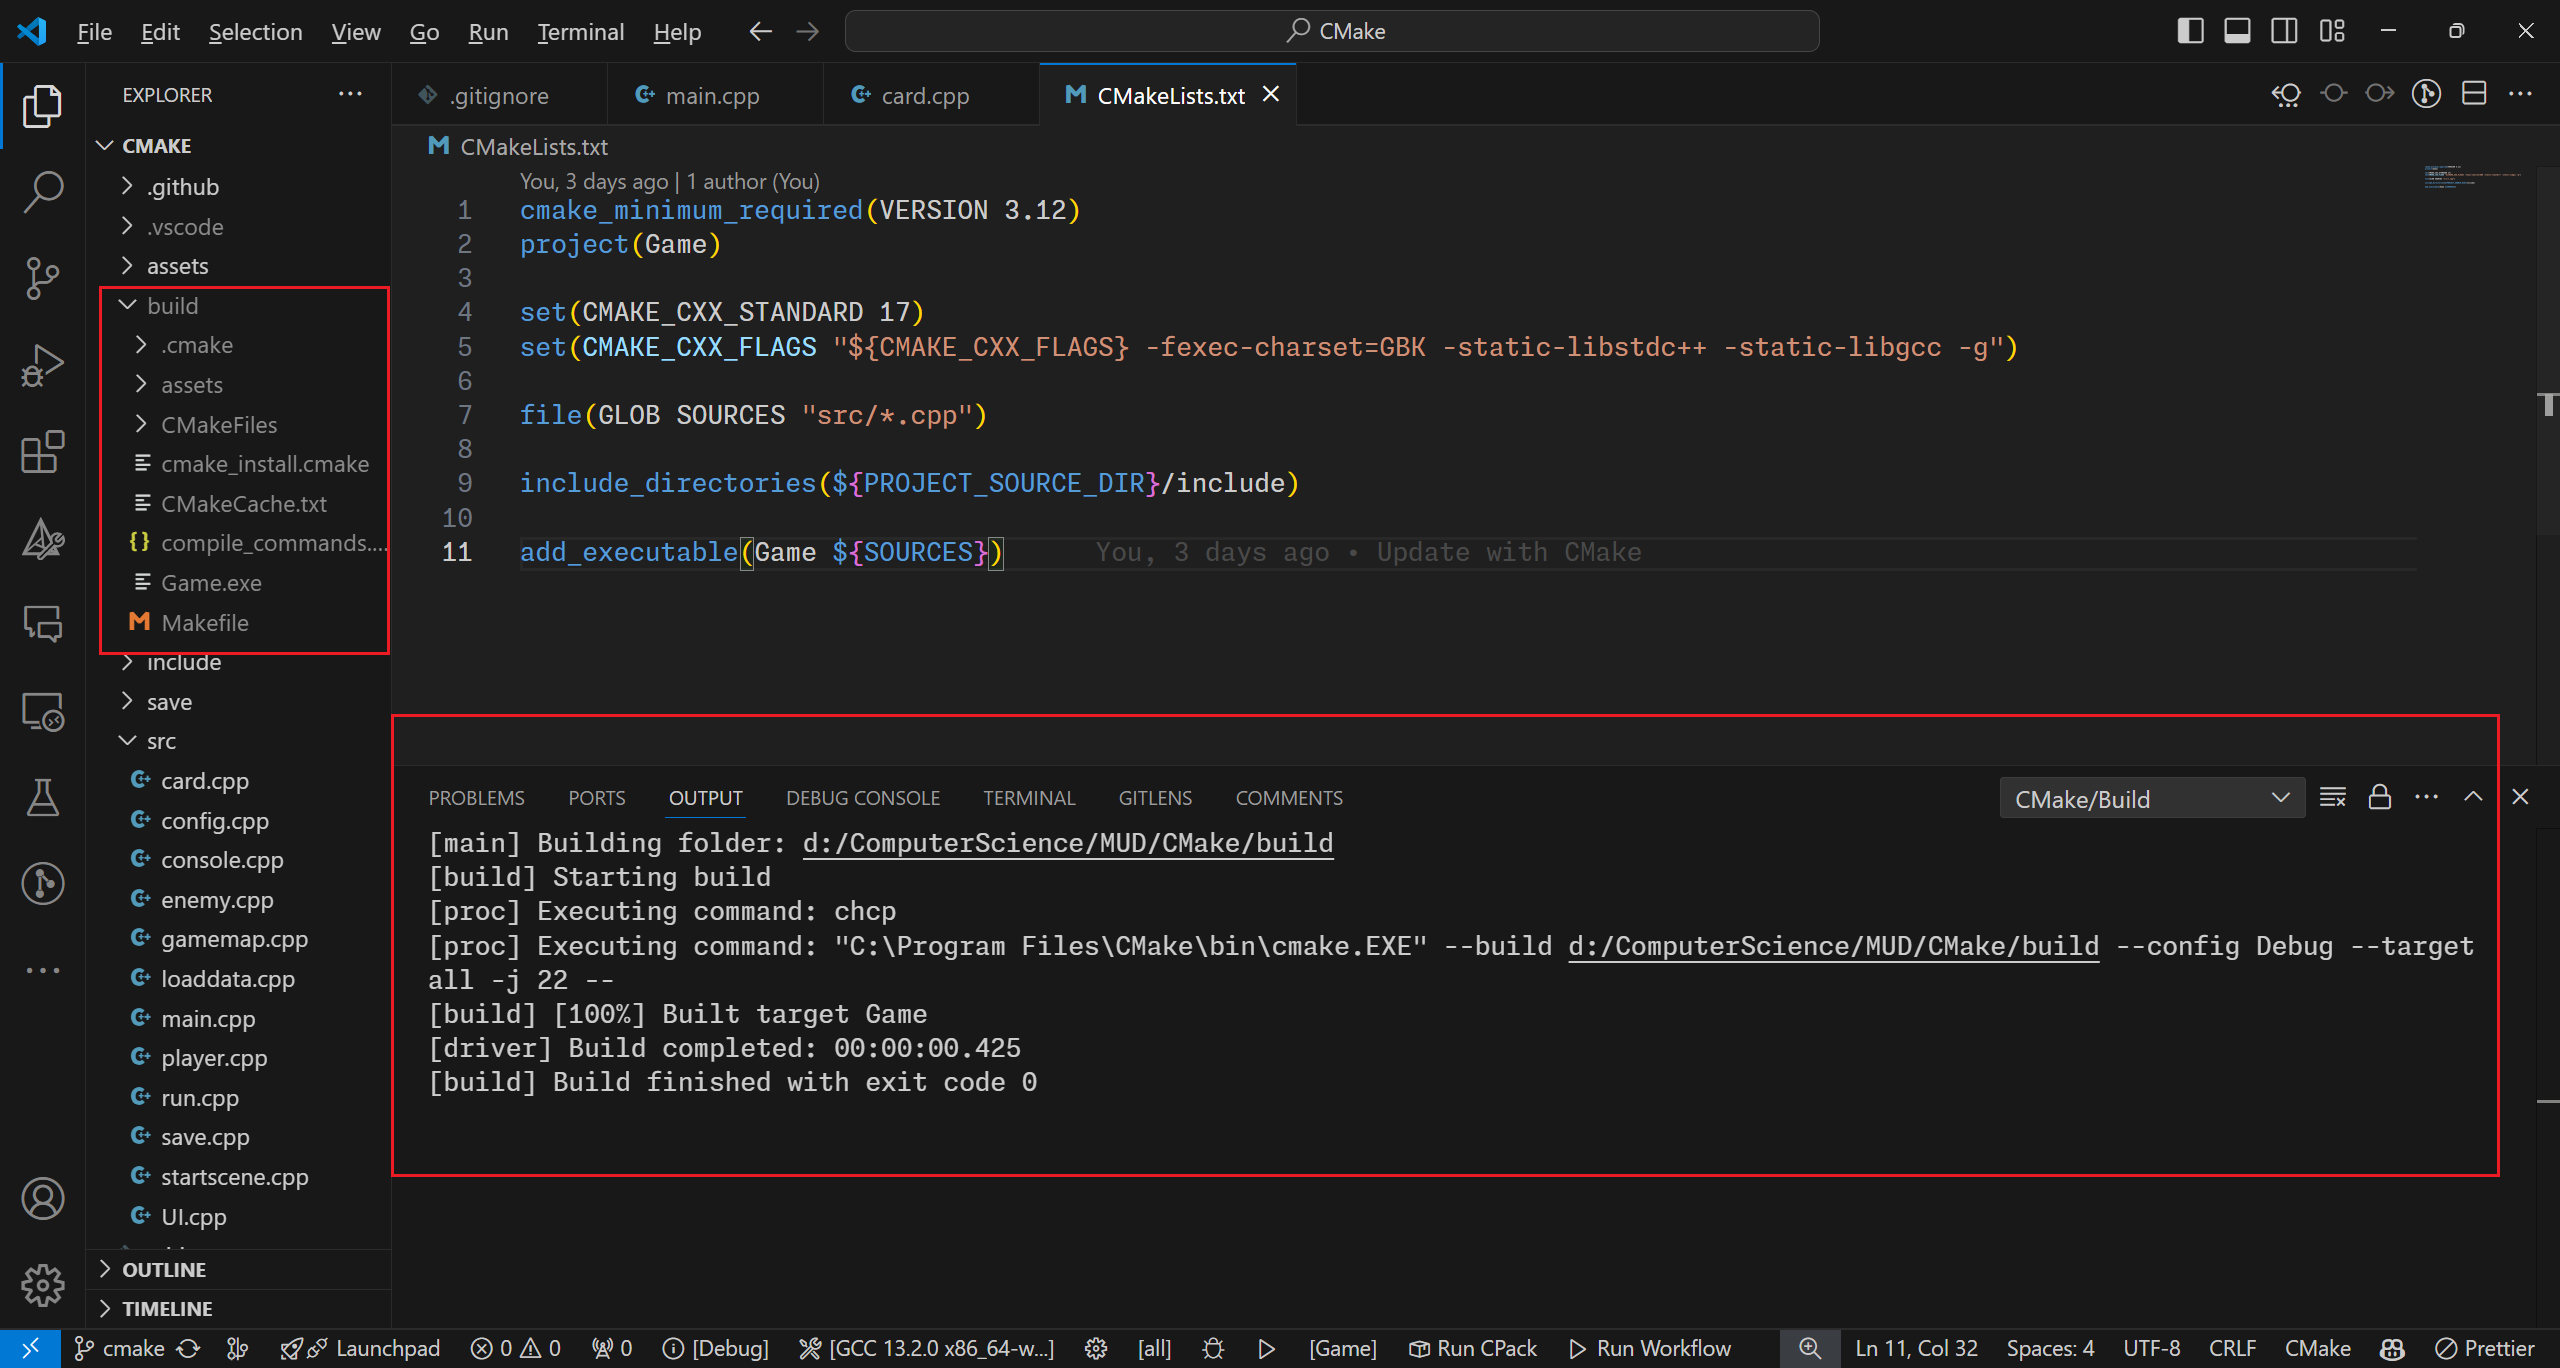
\includegraphics[width=0.85\textwidth]{Figures/cmake.png}
    \caption{使用CMake构建项目的示例}
    \label{fig:cmake}
\end{figure}

此外,\textbf{在大型项目中,CMake允许开发者将不同的构建任务分成多个CMakeLists文件},方便管理。\textbf{CMake还支持第三方库的查找和自动化集成},例如通过\texttt{find\_package}命令自动查找并链接外部依赖库。对于跨平台项目,\textbf{CMake能够根据不同平台自动调整编译选项和链接方式},使得开发者无需为每个平台单独编写构建脚本。\\

特别地,我们要\textbf{介绍Ninja,这款构建工具类似于Makefile},但是\textit{与传统的Makefile相比,Ninja能够更高效地处理并行编译任务,从而显著减少编译时间}。它正是一款\textbf{与CMake集成良好的工具,专为提高大规模项目的构建速度而设计。}在实际开发中,使用\texttt{cmake -G Ninja}可以生成\texttt{Ninja}的构建文件。

\section{持续集成系统}

\subsection{概述}

\textbf{持续集成(Continuous Integration, CI)是一种软件开发实践},其核心思想是\textit{频繁地将代码集成到主干分支,通过自动化构建和测试,尽早发现和解决代码集成引入的问题}。持续集成的目标是\textit{减少开发周期,提高软件质量,降低风险}。持续集成系统是实现持续集成的关键工具,可以\textit{自动化构建、测试和部署过程,提高开发效率和代码质量}。

\subsection{GitHub Action}

\textbf{GitHub Action是GitHub提供的一款持续集成工具},它允许开发者\textit{在GitHub仓库中配置自动化构建、测试和部署任务}。GitHub Action的核心概念是\textit{Workflow},即一组自动化任务的有序执行流程。每个Workflow由一个或多个\textit{Job}组成,每个Job包含一个或多个\textit{Step}。每个Step是一个独立的任务,可以是构建、测试、部署等操作。\\

我们在夏季小学期的项目中,实际上在完成CMake构建后,就用了\textit{GitHub Action}来自动化构建和测试我们的项目。我们的\texttt{.github/workflows}目录下的\texttt{cmake-single-platform.yml.yml}文件如代码\ref{listing:github-action}所示。

\begin{longlisting}
    \begin{minted}{yaml}
name: CMake on a single platform

on:
  push:
    branches: [ "main" ]
  pull_request:
    branches: [ "main" ]

env:
  # Customize the CMake build type here (Release, Debug, RelWithDebInfo, etc.)
  BUILD_TYPE: Release

jobs:
  build:
    # Runs on Windows platform
    runs-on: windows-latest

    steps:
    # Step 1: Check out the code from the repository
    - uses: actions/checkout@v4

    # Step 2: Install necessary dependencies
    - name: Install Dependencies
      run: |
        choco install cmake
        choco install ninja  # If using Ninja generator, you can adjust based on your needs

    # Step 3: Configure CMake (use the 'build' directory)
    - name: Configure CMake
      run: cmake -B ${{github.workspace}}/build -S ${{github.workspace}} -G "Ninja" -DCMAKE_BUILD_TYPE=${{env.BUILD_TYPE}}

    # Step 4: Build your project using CMake
    - name: Build
      run: cmake --build ${{github.workspace}}/build --config ${{env.BUILD_TYPE}}

# Step 5: Run tests using CTest
    - name: Test
      working-directory: ${{github.workspace}}/build
      run: ctest -C ${{env.BUILD_TYPE}} --output-on-failure

    - name: Prepare Artifacts
      run: |
        mkdir "${{github.workspace}}/artifacts"
        copy "${{github.workspace}}\\build\\Game.exe" "${{github.workspace}}\\artifacts\\Game.exe"
        xcopy /E /I "${{github.workspace}}\\assets" "${{github.workspace}}\\artifacts\\assets"

    - name: Upload Artifacts
      uses: actions/upload-artifact@v4
      with:
        name: game-build
        path: ${{github.workspace}}/artifacts
    \end{minted}
    \caption{GitHub Action配置文件示例}
    \label{listing:github-action}
\end{longlisting}

在其中包含了\textit{自动安装CMake、Ninja、配置CMake、构建项目、运行测试、准备构建产物和上传构建产物}等步骤。具体运行效果见图\ref{fig:github-action}。

\begin{figure}[!htbp]
    \centering
    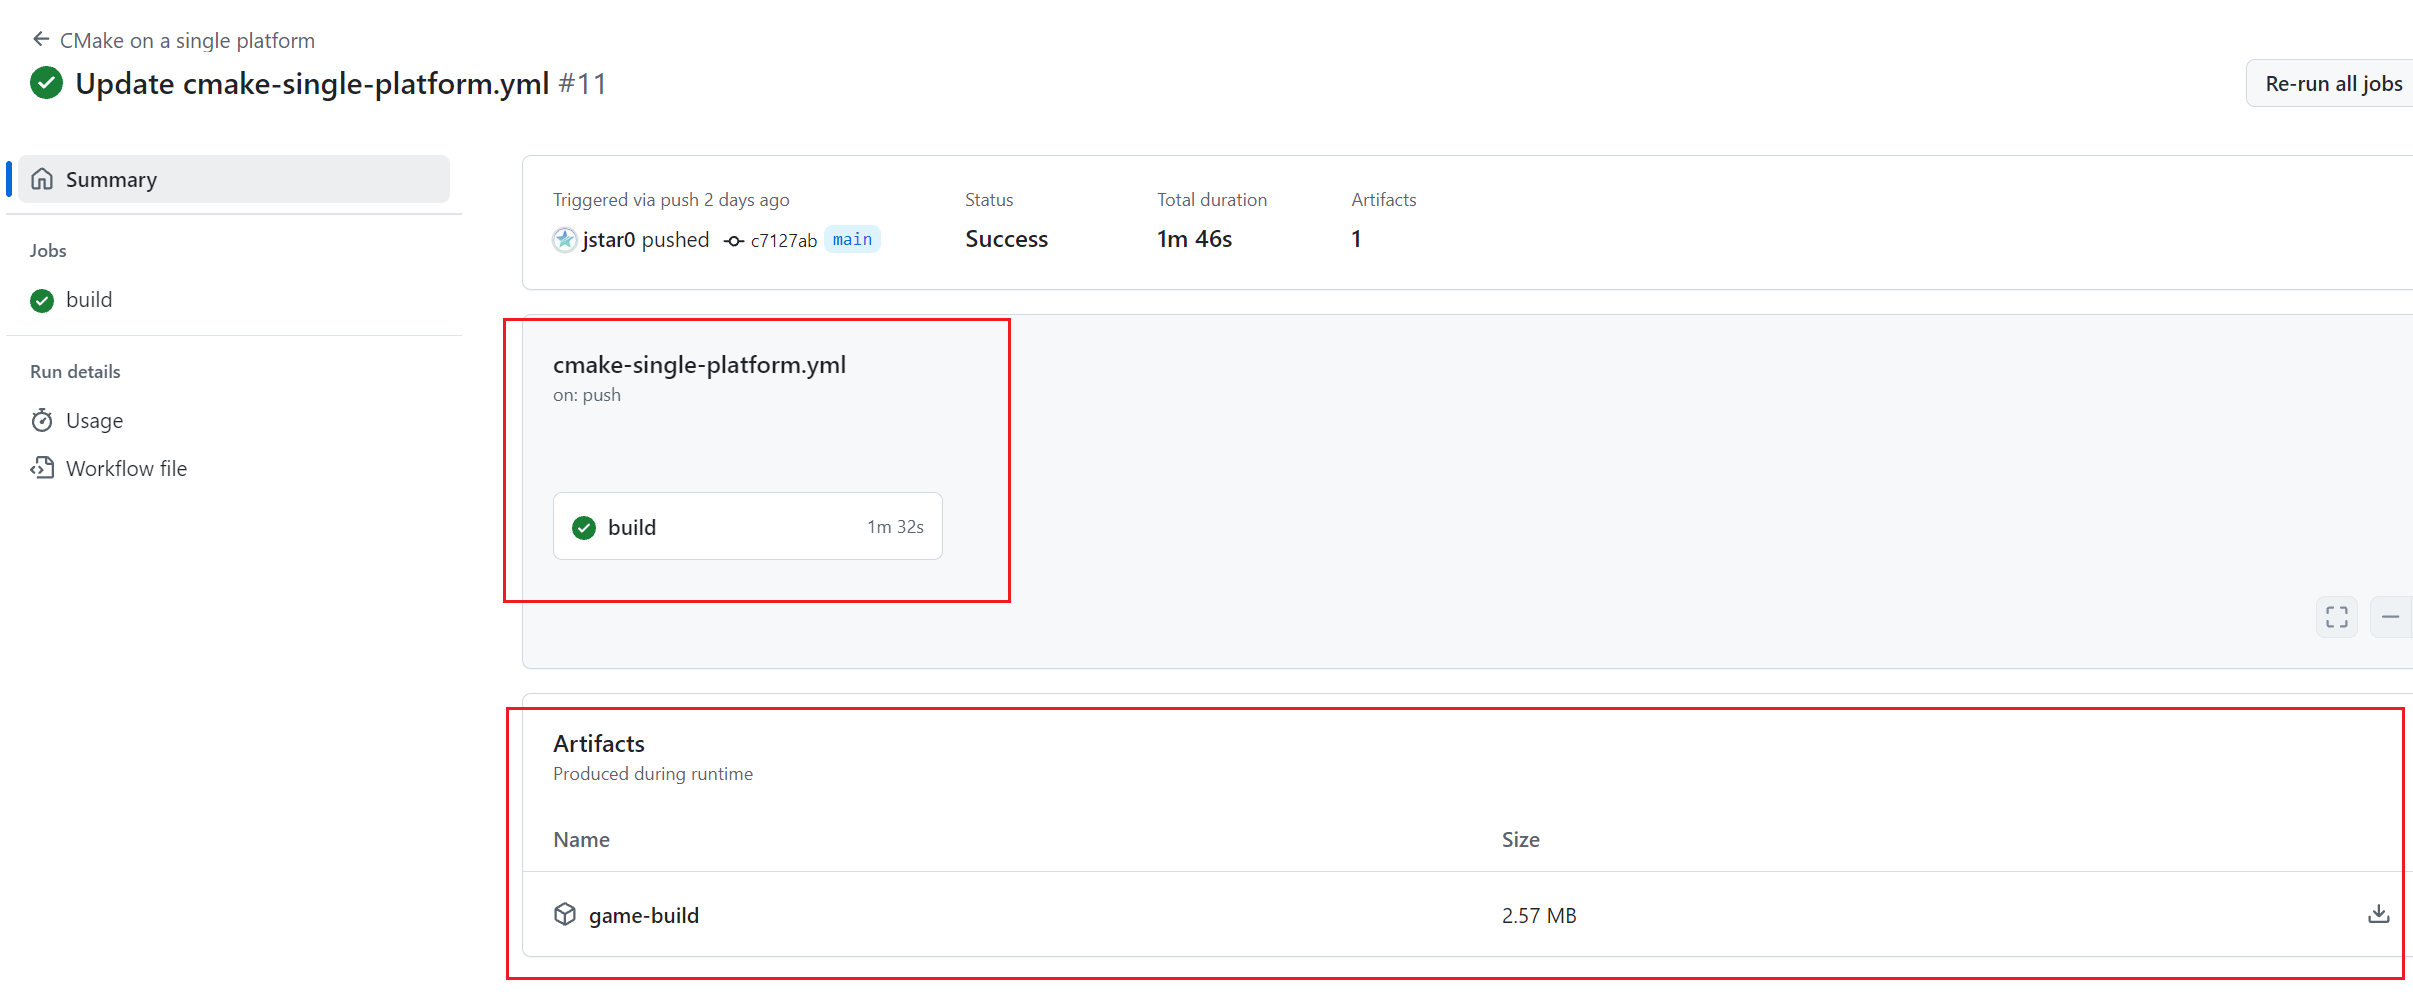
\includegraphics[width=\textwidth]{Figures/github-ci.png}
    \caption{使用GitHub Action构建项目的示例}
    \label{fig:github-action}
\end{figure}

您也可以前往\href{https://github.com/jstar0/CppGame/actions/workflows/cmake-single-platform.yml}{Repo Workflows 页面}查看具体的运行效果。